\section{Experimental Evaluation}


We implemented \toolname in Python 3.8, and Gurobi 9.52 was used for solving LP and MILP problems. We conducted our evaluation on an AMD 5975WX  ($32$ cores$@3.6$GHz, 7nm, year 2022) 
with 256 GB of main memory and an NVIDIA RTX 3090 (not used for CMP). 


We conducted our evaluation on neural networks obtained from the ERAN GitHub (\url{https://github.com/eth-sri/eran}, the 4th to the 8th DNNs provided).
These verification-agnostic DNNs have varying sizes: $5\times 100$, $5\times 200$, $8 \times 100$, $8 \times 200$ and $6 \times 500$. We selected the 4 first because they have been tested in both \cite{prima} and \cite{crown}, they have good accuracy ($>94\%$ \cite{prima}), 
and depite their small sizes there is still a large portion ($12\%$ to $20\%$) of images which are {\em undetermined} by these SOTA methods, that is images neither verified nor for which an attack has been found  \cite{attack}. Hence more accurate methods are useful. 
The next DNN in the list was the larger $6 \times 500$ DNN, which seemed an interesting challenge (very high accuracy and few attacks) to understand the scaling of CMP. Interestingly, tests on $6 \times 500$ were not reported in \cite{prima} nor in \cite{crown}. All these DNNs tackle the MNIST benchmark, which is not a limitation as we want to validate that focusing on compensating strength improves the accuracy: we do not claim that the particular CMP implementation is the most efficient in all the situations.

To obtain results comparable with \cite{prima,crown}, 
we evaluated CMP on $5\times 100$, $5\times 200$, $8 \times 100$, $8 \times 200$ for the first 1000 images of the dataset. For $6\times 500$ (results not reported in \cite{prima,crown}), we run all the tools ourselves for the first 200 images, given the computational overhead associated with such larger network. Each DNN is associated with a $\varepsilon>0$ for the $L^\infty$ norm.

\smallskip

\noindent{\bf Baseline}: 
We compare the following verifiers performing value-abstraction:
\begin{itemize}
	\item DeepPoly \cite{deeppoly}/ CROWN \cite{crown}. We report the runtime from our  implementation in CMP. 
	%It shows that our purely Python implementation is not optimal ($10$ to $100$ times slower than the implementation in ($\alpha$)($\beta$)CROWN, ERAN and PRIMA). 
	\item PRIMA~\cite{prima} and $(\alpha)\beta$ CROWN \cite{crown}. We use the results reported in \cite{prima} and \cite{crown} respectively for 
	$5\times 100$, $5\times 200$, $8 \times 100$, $8 \times 200$.
	We report our experimental results for the $6\times500$ DNN as they are not available in prior work. Notice that PRIMA and CROWN use massively parallel (>4000 threads) GPUs, and run 16 CPU threads for the first 4 benchmarks, compared with 20 CPU threads and no GPU for CMP.
	\item We also tested MN-BaB \cite{ferrari2022complete} on $6\times500$
	(slightly lower accuracy and slower than $\alpha$,$\beta$-CROWN), 
	in line with results reported in \cite{ferrari2022complete} for other DNNs. Further, results for MN-BaB on $5\times 100$, $5\times 200$, $8 \times 100$, $8 \times 200$	are not reported in \cite{ferrari2022complete} or elsewhere. 
	We thus do not include MN-BaB results in Table \ref{tab:example}, to avoid clutter.
%	They use GPU while we do not. When computing the whole correlated space, 
%	parallelization is difficult.
%	Notice that on these DNNs, PRIMA resort to refined bounds on the first few layers (3 or 4) using exact MILP encoding of all the nodes (which is easily parallelized - 16 nodes considered in parallel in PRIMA). This is doable on the first few layers as the number of integer variable is not too large. By comparison, we run MILP on all the layers, but with a bounded number of integer variables to control the runtime and to scale to all the layers.
%	Its main idea is to implement a very efficient Branch and Bound (BaB) verification tool, subsuming BaBSR \cite{BaB}, and using GPU implementation (while we do not). Performance of pure BaB on these 
%	"hard to verify" DNNs is however impaired by the large number of branchs to consider. Similarly as PRIMA, $\beta$-CROWN resorts to refining the bounds of the first few layers using an exact MILP encoding, also computing 16 nodes in parallel, before running the branching heuristic BaB-FSB. 
%	\item We also experimented with the latest versions of $\alpha$-$\beta$-CROWN (October 2023) and PRIMA (2022) on MLP $6 \times 500$ (results not reported in \cite{crown,prima}).
	\item We do not report results from kPoly \cite{kpoly}, OptC2V \cite{optC2V}, 
	SDPFO \cite{SDPFI}, MIPplanet \cite{MIPplanet}, as $(\alpha)\beta$-CROWN has been shown to outperform these methods in accuracy and time \cite{crown}.
	
\end{itemize}



The  objectives of our evaluation was to answer the following  questions:

\begin{enumerate}
	\item How does the the choice of the set $Z$ impacts the accuracy of $\MILP_Z$? 
	\item Can compensating strength, as implemented in CMP, outperform accuracy of the SOTA? 
\end{enumerate}

\subsection{Utility of Heuristic based on Compensation Strength  }

%The first group of experiments we run, tests the accuracy of choosing a set $Z$ of $K$ nodes using compensation strength, compared with randomly choosing the same number $K$ of nodes,  to understand if the choice is meaningful or any set $Z$ with the same size will result in a similar accuracy.
To measure the impact of the heuristic based on compensation strength, we focused on the smallest DNN (i.e. $5\times 100$) so as to obtain exact bounds for the first few layers using a full MILP encoding of the DNN. We tested over the $\vx=59$th image in the MNIST dataset, as it has a large number of unstable ReLU nodes in the first few layers ($61$ in the first and $55$ in the second layer), so we can experiment with a larger choice of values) for $K$.

To measure the accuracy, we measure the uncertainty of all nodes in a layer:
the uncertainty of a node is the range between its computed lower and upper bound. 
We then average the uncertainty among all the nodes of the layer.
Formally, the uncertainty of a node $n$ with bounds $[\alpha,\beta]$ is $unc(a) = \beta - \alpha$. The average uncertainty of layer $\ell$ is $\dfrac{\sum_{a\in l} unc(a)}{size(\ell)}.$







%KSM: I don't think this is really the place for the paragraph below
% Let $c$ be a node of the second layer.
%A compensating pair $(\pi,\pi')$ of paths with target $c$ is thus of the form a node $a b c$ and $a b' c$, with $a$ an input node and $b,b'$ on the first layer. The compensating strength for $(b,b')$ is defined as $comp(b,b')=\sum_a \val_{\vx}(a) \min(weight(abc),weight(ab'c))$. Indeed, the pair $(a b c,a b' c)$ of path cannot compensate more than $\val_{\vx}(a) \min(weight(a,b,c),$\newline $weight(a,b',c))$, and $b,b'$ would help compensated the set of pairs of paths $\{(a b c,a b' c) \mid a$ is in the first layer$\}$. After selecting the heaviest $(b_0,b_0')$, we can then compute $comp(b)= \sum_{b' \text{already selected}} comp(b,b')+comp(b',b)$ and select iteratively the heaviest $b$'s one by one till reaching the threshold. 
%We do this for all node $c$ of the second layer.

\iffalse

\subsubsection*{ReLU Node in the first hidden layer}


We first focus on the choice of nodes in the first hidden layer, and its consequences on the accuracy of nodes in the second layer. 
We report in Table \ref{tab:example0} the average uncertainty of $\MILP_Z$ following the choice of the $K$ heaviest compensating ReLU nodes in $Z$, vs choosing $K$ nodes randomly. The range of uncertainty created by inacurate computations is up to $1.17=2.22-1.05$, $2.22$ being the accuracy provided by LP, and $1.05$ by an exact MILP encoding of all the unstable ReLU nodes. Selecting $30$ out of the $61$ unstable ReLU nodes, the uncertainty created by inacurracies is reduced by $80\%$, while a random choice of nodes only leads up to roughly halving this number. We can deduce that selecting nodes based on compensating strength helps to select important ReLU nodes for the accuracy.



\begin{table}[h!]
	\centering
	\begin{tabular}{|c||c|c|}
		\hline
		\text{Number $K$ of nodes in $Z$}  &  \text{Compensate strength} & \text{Random Choice}  \\ \hline
		\hline
		0  &  2.22 & 2.22  \\ \hline
		10  &  1.84 & 2.03  \\ \hline
		20  &  1.50 & 1.82  \\ \hline
		30  &  1.28 & 1.62  \\ \hline
		40  &  1.14 & 1.44  \\ \hline
		50  &  1.06 & 1.23  \\ \hline
		61 (max) & 1.05 &  1.05 \\ \hline
	\end{tabular}
	\caption{Average uncertainty of $\MILP_Z$ for nodes of the second layer, for $Z$ with $K$ ReLU nodes of the first layer (compensating strength vs random choice).}
	\label{tab:example0}
	%\vspace{-0.8cm}
\end{table}




\subsubsection*{ReLU Node in the first and second hidden layer}
\fi


\begin{table}[t!]	
	\centering
	\begin{tabular}{|c||c|c|c|}
		\hline
		\text{Number $K$}  &  \text{Compensate} &  \text{Incoming Weights} \cite{9211410} & \text{Random} \\ \hline
		\hline
		0  &  1.761 & 1.761 & 1.761  \\ \hline
		10  &  1.641 & 1.651 & 1.696  \\ \hline
		20  &  1.517 & 1.557 & 1.619  \\ \hline
		30  &  1.392 & 1.489 & 1.546  \\ \hline
		40  &  1.275 & 1.447 & 1.469  \\ \hline
		50  &  1.158 & 1.426 & 1.388  \\ \hline
		116 (max) &  0.895 & 1.424 (max=$61$) & 0.895  \\ \hline
	\end{tabular}
	\caption{Average uncertainty of $\MILP_Z$ for nodes of the third layer, for $Z$ with $K$ ReLU nodes of the 1st and 2nd layer (compensating strength vs \cite{9211410} vs random choice).}
	\label{tab:example1}
	\vspace{-0.6cm}
\end{table}



We focus on the uncertainty of nodes in the third layers, wrt ReLU nodes in the first and second layer. The bounds for nodes of the first two layers are computed exactly using the full MILP encoding. Let $d$ be a neuron of the third layer.
We let $\delta_{\pi,\pi'}=1$ if $(\pi,\pi')$ is compensating, 0 otherwise.
We evaluate the pair $(c,c')$ of nodes in the previous (second) layer in the following way: let $comp(c,c')=\sum_{b} \delta(bcd,bc'd) \val_{\vx}(b) \min( weight(bcd),weight(bc'd))$, meaning that we take into account all the sources $b$ such that $(bcd,bc'd)$ is compensating. 

We select the pair $(c,c')$ with the highest $comp(c,c')$, and let $Z=\{c,c'\}$.
Then, we add nodes iteratively to $Z$, starting with the highest $comp(c)=\sum_{c' \in Z} comp(c,c')$. Further, we can add nodes $b$ from the first layer, taking into account compensating pairs $(a b c d, a b' c' d)$ for all $\{c,c'\} \in C$. 
Let $comp(b,b')=\sum_a \sum_{c,c' \in Z} \delta(abcd,ab'c'd) \val_{\vx}(a) \min( weight(abcd)$, $weight(ab'c'd))$ and add $b,b'$ to $Z$ with the highest $comp(b,b')$.
We then let $comp(b)=\sum_{b' \in Z} comp(b,b') + comp(b',b)$, and iteratively select nodes $b$ (first layer) or $c$ (second layer) by selecting the heaviest $comp(b)$ or $comp(c)$. The intuition behind the formula is straightforward: $\val_{\vx}(a)weight(abcd)$ is the contribution from node $a$ to the target $d$ using $weight(abcd)$, and min of two paths is a natural value to represent the strength of compensation: if one of them is very small, the effect of compensation will also be very small.

We report in Table \ref{tab:example1} the average uncertainty of $\MILP_Z$ following the choice of the $K$ heaviest compensating ReLU nodes in $Z$, vs choosing $K$ nodes from layers $1$ and $2$. We test using compensation, compared with a random choice, and also choice based on strength in \cite{9211410}, defined as $strength(c) = (UB(n)-LB(n))\cdot W_{cd}$. It is however limited to choosing ReLU in the previous layer 2. This choice is fine for few nodes (10,20), as there is a high correlation between $comp(c)$ being high and $W_{cd}$ being high. However, as soon as many nodes can be chosen in $Z$, compensate becomes much more accurate. Even random becomes more accurate as the number of nodes grows, as \cite{9211410} only has access to nodes $c$ in layer 2, and not to nodes $b$ in layer 1.
For comparison, compensate is the most accurate, from 30 nodes, experimentally validating that compensating strength is the important factor to consider. 

\iffalse
Choosing ReLU nodes in the previous layer (layer $2$) only is less accurate than 
also choosing nodes in layer $1$. When picking in both layer $1$ and $2$, choosing $50$ out of $116$ unstable ReLU nodes allows to reduce by $90\%$ the average uncertainty due to inaccurate computations ($0.059$ vs $0.574$), while it only reduces the uncertainty by $65\%$ when choosing nodes randomly. Notice that applying this layer after layer will even further reduce uncertainty created by accumulation of inaccuracies. 
Last, we did not experiment for selecting ReLU nodes in 3+ layers earlier because the trade-off of accuracy vs evaluating the compensating strength of such paths is unclear.

{\color{red} We report in Table \ref{tab:example1} the average uncertainty of $\MILP_Z$ following the choice of the $K$ heaviest compensating ReLU nodes in $Z$, vs choosing $K$ nodes randomly from layers $1$ and $2$. 
	Moreover, we also compare choosing nodes in the second layer only (using method in paper \cite{9211410}) with choosing nodes in both the first and second layer.
	
	
		The method in paper \cite{9211410} use a formula to value different nodes in a layer, and then choose nodes by their values. We can use the same formula in this comparison experiments. Because we only have $\ReLU$ function, that formula can be simplified to: $$V(n) = (UB(n)-LB(n))\cdot W_{nm}.$$ In this formula, $m$ is the target node, and $n$ is one of source nodes in one layer before. We sort all nodes $n$ by their $V(n)$ values, and choose the nodes with larger values. 
	
	
	
	Choosing ReLU nodes in the previous layer (layer $2$) only is less accurate than 
	also choosing nodes in layer $1$. 	When picking in both layer $1$ and $2$, choosing $50$ out of $116$ unstable ReLU nodes allows to reduce by $90\%$ the average uncertainty due to inaccurate computations ($0.059$ vs $0.574$), while it only reduces the uncertainty by $65\%$ when choosing nodes randomly. Notice that applying this layer after layer will even further reduce uncertainty created by accumulation of inaccuracies. 
	Last, we did not experiment for selecting ReLU nodes in 3+ layers earlier because the trade-off of accuracy vs evaluating the compensating strength of such paths is unclear. 
	
}
\fi



\newcolumntype{C}{>{\centering\arraybackslash}X}







\subsection{Comparison with Prior State of the Art}

We present the accuracy analysis of various techniques in Table~\ref{tab:example}, and provide runtime for reference. Further, for each DNN, a PGD-attack \cite{attack} is run 
on all the images. We report the $\%$ of images without attack, giving an {\em Upper Bound} on the $\%$ of images that can be certified.

Several observations are noteworthy: DeepPoly (or CROWN) is by far the fastest, yet it is also the least accurate, certifying robustness for fewer than $30\%$ of the images. In contrast, there are at least $82\%$ of the images for which no attack is found. Similarly, PRIMA achieves better accuracy than DeepPoly/CROWN but falls short of \toolname. 

Next, we shift focus to the comparison with ($\alpha$)$\beta$-CROWN, where we observe intriguing trade-offs. On the shallowest DNNs (5 layers, $5 \times 100$, $5 \times 200$), \toolname accuracy is close to $\beta$-CROWN, within 1.5\%. Here, RefinedBaB used by $\beta$-CROWN, has the time to refine most of the nodes, and thus the number of branches BaB has to explore is small enough that it is very accurate.
As the network size increases, \toolname demonstrates better accuracy in comparison to $\beta$-CROWN: For $8 \times 100$ and $8 \times 200$, 
RefinedBaB used by $\beta$-CROWN can only consider half of the layers. 
On many images, there are too many branches for BaB left to consider, and it times-out.
As expected, there's a trade-off between runtime and accuracy: \toolname can verify more images, albeit with increased computation time. Overall, on $8 \times 200$, CMP closes the gap of {\em undetermined} images from $17.6\%$ ($\beta$-CROWN) to $10.4\%$ (CMP).


\begin{table}[t!]
	\centering
	\begin{tabularx}{\textwidth}{|C||C||C|C|C||C|}
		
		\hline
		\text{DNN} & \shortstack{Upper\\Bound} & \shortstack{DeepPoly/\\CROWN} & PRIMA & \shortstack{($\alpha$)$\beta$-\\CROWN} & \toolname \\ 
		\hline \hline
		
		$5 \times100$\  & $84.2 \%$ & $16\%$ & $51\%$ & $\mathbf{69.9\%}$ & $68.4\%$\\ 
		$\epsilon = 0.026$ &  & 5s & 159s & 102s & 142s\\
		\hline	
		
		$5 \times 200$ \  & $90.1 \%$ & $18.2\%$ & $69\%$ & $\mathbf{77.4\%}$ & {$76.8\%$}\\ 
		$\epsilon = 0.015$ &  & 11s & 224s & 86s & {279s} \\ \hline \hline
		
		
		$8\times100$\  & $82.0 \%$ & $29.2\%$ & $42.8\%$ & $62\%$ & {$\mathbf{65.8\%}$}\\ 
		$\epsilon = 0.026$ &  & 8s & 301s & 103s & {346s}\\
		\hline
		
		$8\times200$\  & $91.1 \%$ & $25.9\%$ & $62.4\%$ & $73.5\%$ & {$\mathbf{80.7\%}$}\\ 
		$\epsilon = 0.015$ &  & 17s & 395s & 95s  & {697s}\\ \hline \hline
		
		$6\times500$\  & $92\%$ & $26\%$ & $32.5\%$ & $41\%$ & {$\mathbf{65\%}$}\\ 
		$\epsilon = 0.035$ &  & 34s & 119s & 18.4s & {925s} \\ \hline 
		
	\end{tabularx}
	
	\caption{$\%$ of verified images and average runtime in seconds.
		Results for PRIMA, $\beta$-Crown and the upper bound on the $\%$ are from \cite{crown}, except for $6 \times 500$ for which we run every verifier ourselves.
	}
	\vspace{-0.8cm}
	\label{tab:example}
\end{table}





The last network $6 \times 500$ (verification-agnostic) is the largest one. 
Results for CMP are good, at $65\%$ of verified images, comparable with $8\times 100$, taking less than $0.3s$ per neuron to perform the verification in average per image (there are more neurons, so longer runtime was expected). For comparison, results for $6 \times 500$ were not reported in \cite{crown,prima}. On this larger network, it is unclear whether the {\em refined strategy} of PRIMA and of $(\alpha)\beta$-CROWN is applicable, as the number of binary variables to encode even the first few layers is very large. As a matter of fact, refinedBaB is "NotImplemented" in $(\alpha),\beta$-CROWN for this network, and the results are surprisingly inaccurate and fast in refinedPRIMA (even faster than for $5 \times 100$), probably because few/no nodes are actually refined. We thus resort and reported the standard pureBaB setting of $\alpha,\beta$-CROWN, with the usual 30s timeout. Accuracy on $\alpha,\beta$-CROWN is very low, only $15\%$ more images verified than DeepPoly. 
We also tested $\alpha,\beta$-CROWN with longer time-out, to understand $\alpha,\beta$-CROWN scaling. With time-out=$2000s$, the runtime of $\alpha,\beta$-CROWN is $954s$, comparable with $925s$ for CMP. This only improved the accuracy of $\alpha,\beta$-CROWN by $3.5\%$, at $44.5\%$, with a runtime $50$ times longer. We conclude that the number of branches is often too high for $\alpha,\beta$-CROWN to tackle such a hard verification-agnostic DNN. We also experimented MN-BaB \cite{ferrari2022complete} on $6 \times 500$. Results were similar to $\alpha,\beta$-CROWN: $40\%$ (18s) [30s Time-out] and $43\%$ (1036s) [2000s Time-out]; within 1.5\% of $\alpha,\beta$-CROWN. For comparison, CMP could verify more than $20\%$ more images than $\alpha,\beta$-CROWN (or MN-BaB) with similar runtime (around 17min per image).




% BaB focuses on the output neuron, computing bounds for it, and refining the different ReLU as necessary. Instead, we consider every node one by one from the input layer till the final layer, with the same accuracy. Hence {\toolname} will spend a lot of time on nodes which are not necessary for the verification. 
% 
%It is worth remarking that our prototype implementation (in Python)  Therefore, our naive implementation is not as efficient as the highly optimized $\beta$-CROWN: our slow setting is $1.4$ to 
%$6.5$ times slower than $\beta$-CROWN. Notice {\toolname} it is not using GPUs. 
%Concerning accuracy: on shallower DNNs ($5 \times 100$ and $5 \times 200$ with $5$ hidden layers), refined BaB uses MILP on all but the last $2$ layers, leaving BaB with few ReLU nodes to branch on, and $\beta$-CROWN (refined BaB) is slightly more accurate than using the slow fixed setting of {\toolname}, with a small difference of less than $1.5\%$. On deeper DNNs ($8 \times 100$ and $8 \times 200$ with $8$ hidden layers), the full MILP used in refined BaB cannot treat the last $4$ layers, and BaB has more ReLU nodes to branch on: 
%the most accurate setting (slow fixed) of {\toolname} is more accurate than $\beta$-CROWN, closing the gap with the upper bound from $20\%$ to $16.2\%$ ($8 \times 100$)
%and from $17.6\%$ to $10.4\%$ ($8 \times 200$). This is very promising for the compensation idea, which could be used in many different ways than in {\toolname} (see Section \ref{Discussion}).

%Further, unlike PRIMA, we do not resort to a GPU, and our purely Python implementation is not optimal. This is very promising for this idea of compensation, which indirectly treats dependencies between the variables, which PRIMA represents explicitly.





%In Table \ref{tab:example}, we report the accuracy and runtime of these different methods.
%DeepPoly/CROWN is by far the fastest, but also the most inaccurate, certifying robustness for less than $30\%$ of the images, whereas there are at least $82\%$ of the images for which no attacked is found (attacks computed by \cite{attack} in $\beta$-CROWN).
%This is because these DNNs, although of reasonable size, are hard to verify (they are trained in a natural way, with high compensation strength, see Section \ref{Sec.comp}).


%Compared with PRIMA (using refinement of the first few layers by exact MILP), the overall pipeline is quite similar, looking at all the nodes one by one from the beginning of the network till the end. 
%Now, moving on to PRIMA, our 
%Our method compare favorably, both in terms of time and accuracy: our fast adaptive setting is always faster than PRIMA, sometimes by a large margin ($>3$ times faster on $8 \times 100$ while verifying $10\%$ more images), and also more accurate (except for $5 \times 200$ which is quite pointless on this shallow DNN - the fast fixed method is both faster and more accurate than PRIMA), sometimes by a large margin (by $14 \%$  for $5 \times 100$ while being $30\%$ faster). Further, unlike PRIMA, we do not resort to a GPU, and our purely Python implementation is not optimal. This is very promising for this idea of compensation, which indirectly treats dependencies between the variables, which PRIMA represents explicitly.



%\begin{table}[t!]
%	\centering
%	\begin{tabular}{|c||c|c|c||cc|cc||c|}
%		
%		\hline
%		\text{DNN}  & DeepPoly & PRIMA & $\beta$-CROWN &\multicolumn{2}{@{}c@{}|}{\color{blue}\text{ Comp (adapt.) }} & \multicolumn{2}{@{}c@{}|}{\color{blue} \text{ Comp (fixed) }} & Upper\\ 
%		& / CROWN & (refined) & (refined BaB) & {\color{blue}fast} & {\color{blue}slow} & {\color{blue}fast} &{\color{blue}slow} & Bound\\
%		\hline \hline
%		
%		$5 \times100$\  &   $16\%$ & $51\%$ & $\mathbf{69.9\%}$ & {\color{blue}$57.5\%$} & {\color{blue}$66.1\%$} & {\color{blue}$65.3\%$} & {\color{blue}$68.4\%$} &  $84.2 \%$ \\ 
%		$\epsilon = 0.026$ & 5s & 159s & 102s& {\color{blue}75s} & {\color{blue}140s} & {\color{blue}117s} & {\color{blue}142s} &  \\
%		\hline	
%		
%		$5 \times 200$ \  &  $18.2\%$ & $69\%$ & $\mathbf{77.4\%}$ & {\color{blue}$64.3\%$} & {\color{blue}$74.7\%$} & {\color{blue}$72\%$} & {\color{blue}$76.8\%$} & 
%		$90.1 \%$\\ 
%		$\epsilon = 0.015$ & 11s & 224s & 86s & {\color{blue}163s} & {\color{blue}285s} & {\color{blue}206s} & {\color{blue}279s}  &\\ \hline \hline
%		
%		
%		$8\times100$\  &   $29.2\%$ & $42.8\%$ & $62\%$ & {\color{blue}$52.7\%$} & {\color{blue}$59.7\%$} & {\color{blue}$61.4\%$} & {\color{blue}$\mathbf{65.8\%}$}  & $82.0 \%$ \\ 
%		$\epsilon = 0.026$ & 8s & 301s & 103s & {\color{blue}92.3s} & {\color{blue}179s} & {\color{blue}170s} & {\color{blue}346s} & \\
%		\hline
%		
%		
%		$8\times200$\  &   $25.9\%$ & $62.4\%$ & $73.5\%$ & {\color{blue}$68.1\%$} & 
%		{\color{blue}$79.1\%$} & {\color{blue}$72.6\%$} & {\color{blue}$\mathbf{80.7\%}$} & $91.1 \%$ \\ 
%		$\epsilon = 0.015$ & 17s & 395s & 95s  & {\color{blue}297s} & {\color{blue}535s} & {\color{blue}$480s$} & {\color{blue}697s$^\star$} & \\ \hline
%		
%		%6$\times$500\  &   0.035& 1.758 & time & 1.758 & time &    1.758 & time & 1.758 & time & \\ 
%		%$\epsilon = 0.035$ & & & & & & & & & &\\ \hline
%	\end{tabular}
%	\caption{$\%$ of verified images and average runtime in seconds, over 1000 images. 
%		Results for PRIMA, $\beta$-Crown and the upper bound on the $\%$ are from \cite{crown}.
%		\newline $^\star$ For $8 \times 200$, slow fixed results are obtained after running slow adaptative.}
%	\label{tab:example}
%%	\vspace{-1cm}
%\end{table}


%Compared with $\beta$-CROWN (also using a refinement on the first few layers using exact MILP), the picture is more balanced, because the fundamentals of both algorithms are different. BaB focuses on the output neuron, computing bounds for it, and refining the different ReLU as necessary. Instead, we consider every node one by one from the input layer till the final layer, with the same accuracy. Hence {\toolname} will spend a lot of time on nodes which are not necessary for the verification. Therefore, our naive implementation is not as efficient as the highly optimized $\beta$-CROWN: our slow setting is $1.4$ to 
%$6.5$ times slower than $\beta$-CROWN. Notice {\toolname} it is not using GPUs. 
%Concerning accuracy: on shallower DNNs ($5 \times 100$ and $5 \times 200$ with $5$ hidden layers), refined BaB uses MILP on all but the last $2$ layers, leaving BaB with few ReLU nodes to branch on, and $\beta$-CROWN (refined BaB) is slightly more accurate than using the slow fixed setting of {\toolname}, with a small difference of less than $1.5\%$. On deeper DNNs ($8 \times 100$ and $8 \times 200$ with $8$ hidden layers), the full MILP used in refined BaB cannot treat the last $4$ layers, and BaB has more ReLU nodes to branch on: 
%the most accurate setting (slow fixed) of {\toolname} is more accurate than $\beta$-CROWN, closing the gap with the upper bound from $20\%$ to $16.2\%$ ($8 \times 100$)
%and from $17.6\%$ to $10.4\%$ ($8 \times 200$). This is very promising for the compensation idea, which could be used in many different ways than in {\toolname} (see Section \ref{Discussion}).


%KSM: I think this paragraph doesn't make very convincing case. 
%Importantly, ($\alpha$)$\beta$-Crown, while efficient, can face a (complexity) wall, when the number of branches becomes too extreme for BaB to work: either BaB succeds fast, or it will not suceed even with very long timeouts ({\em refined} BaB is more accurate than pureBaB on these networks). We verify that in Table \ref{tab:example3}, on a larger DNN learnt in a natural way, namely MLP $6 \times 500$.
%We tested PureBaB with two timeouts (TO), from standard 30s to an extreme 2000s, to match the average runtime of our adaptative implementation (fast mode). Only $3.5\%$ more images could be ceritifed by extending the TO from 30s to 2000s, certifying $20\%$ less images than our prototype in the same time. Notice that the refined BaB mode of ($\alpha$)$\beta$-Crown (first few layers using MILP) failed to run on this DNN (error code: NoImplementation), and we were unable to fix the problem, which is not really surprising as running exact MILP with so many integer variables is not likely to be efficient, as confirmed while running PRIMA (refined).



% test

%
%\begin{table}[t!]
%	\centering
%	\begin{tabular}{|c||c|c|cc||c||c|}
%		
%		\hline
%		\text{DNN}  & DeepPoly & PRIMA &  \multicolumn{2}{@{}c@{}|}{\text{ $\alpha$-$\beta$-CROWN (pureBaB) \,}} & 
%		{\color{blue}Comp (adapt.)} & Upper\\ 
%		& / CROWN & (refined) & TO=30s & TO=2000s & {\color{blue}fast} & Bound\\
%		\hline \hline
%		$6\times500$\  &   $26\%$ & $32.5\%$ & $41\%$ & $44.5\%$  & {\color{blue}$\mathbf{65\%}$} & $92\%$ \\ 
%		$\epsilon = 0.035$ & 34s & 119s & 18.4s & 954s & {\color{blue}925s} &\\ \hline
%	\end{tabular}
%	\caption{$\%$ of verified images and average runtime in seconds, over 200 images.}
%	\label{tab:example3}
%	
%\end{table}

%\begin{table}[]
%	\centering
%	\begin{tabular}{|c|c|cc||cc||c|}
%		\hline
%		\text{DNN}  & DeepPoly &  \multicolumn{2}{@{}c@{}|}{\text{ $\alpha$-$\beta$-CROWN (refinedBaB) \,}} & 
%		\multicolumn{2}{@{}c@{}|}{\text{ \color{blue}\CMP slow \,}}
%		& Upper\\ 
%		& / CROWN & TO=300s & TO=3000s & {\color{blue}adapt} & {\color{blue}fixed} & Bound\\
%		\hline \hline
%		$8\times200$\  &   $25\%$? & $72\%$? & $\mathbf{79.5\%}$ & {\color{blue}$75.5\%$}  & {\color{blue}$77\%$} & $91\%$ \\ 
%		$\epsilon = 0.015$ & 17s & 95s? & 451s & {\color{blue}391s} & {\color{blue}562s} &\\ \hline
%	\end{tabular}
%	\caption{WIP! $\%$ of verified images over 200 images. To see how refined BAB scale with TimeOut.}
%	\label{tab:example4}
%\end{table}


\iffalse

\subsection{Scalability of {\toolname} with Size of DNNs}

\begin{figure}[b!]
	\centering
	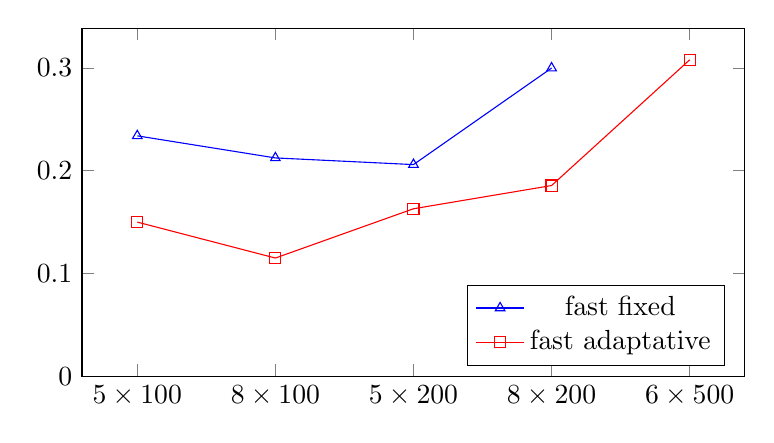
\begin{tikzpicture}
		\begin{axis}[width=10cm,height=6cm,
			xlabel={},
			ylabel={},
			legend pos=south east,
			ymin=0,
			xtick={1,2,3,4,5}, 
			xticklabels={$5\times 100$, $8\times 100$, $5\times 200$, $8\times 200$, $6\times 500$},
			]
			
			
			\addplot[mark=triangle, blue] coordinates {
				(1, 0.234)
				(2, 0.2125)
				(3, 0.206)
				(4, 0.3)
			};
			\addlegendentry{fast fixed}
			
			
			\addplot[mark=square, red] coordinates {
				(1, 0.15)
				(2, 0.115)
				(3, 0.163)
				(4, 0.1856)
				(5, 0.308)
			};
			\addlegendentry{fast adaptative}
			
			
		\end{axis}
	\end{tikzpicture}
	\caption{runtime (seconds per node)}
	\label{fig2}
\end{figure}



We now focus on understanding the potential of {\toolname} for even larger networks than those that are usually considered in the verification community. To this end, Figure~\ref{fig2} presents the  average runtime per node across various DNNS. Observe that while  the average runtime per node isn't fixed (attributable to $\LP(N,K)$), it remains regulated, avoiding exponential increases — from 0.1s per node for the smallest DNN to 0.3s per node for the largest. This suggests that {\toolname} is scalable to larger DNNs, bypassing the high complexity barrier often encountered with approaches such as those based on pure branch and bound.

\fi


\section{Discussion}
\label{Discussion}

CMP ranks highly in terms of accuracy, on the moderately large network (but challenging verification-agnostic) DNNs we experimented with. Even if the CMP complexity is not subject to combinatorial explosion, its runtime, particularly for larger DNNs, can be relatively slow, as CMP needs to consider every node one by one. Tackling much larger networks may thus need different implementation than CMP, while still benefitting from the novel compensation notion we uncovered and validated thanks to CMP. Numerous avenues exist:

A primary strategy involves utilizing $\alpha$-$\beta$-CROWN initially in the sequence, reserving {\toolname} for images unresolved by $\alpha$-$\beta$-CROWN, potentially enhancing this with parallel node computation across additional CPU cores. Another tactic could involve adapting the refined branch-and-bound approach of $\beta$-CROWN to permit {\toolname} to process additional layers beyond MILP's capability, concluding the verification with BaB. More complex strategies might include modifying BaB to branch on unstable ReLU nodes, driven by compensation strength, or analyzing crucial nodes linked to uncertain outputs, enabling quicker computation of less precise bounds for less critical nodes. Furthermore, implementing a Refinement Abstraction framework, akin to methodologies in \cite{atva}, \cite{elboher}, or \cite{SRGR}, could be beneficial.

In terms of neuron correlation, a key feature explicitly encoded by PRIMA, our findings suggest that leveraging compensation strength for network abstraction is generally more effective. Although precise local accuracy is achieved by directly considering ReLU nodes, the accuracy diminishes when correlations originate from distant layers. Retaining a select few significant correlations, in the style of PRIMA, as explicit linear constraints in the MILP model, might offer a strategy to further improve accuracy while keeping the number of binary variables limited. 

Finally, we focused on DNNs employing ReLU activation functions since our approached on usage of MILP, which is naturally suited for ReLU activation function. However, it is worth remarking that the notion of compensation strength is independent of activation function, and therefore, an interesting direction of future work would be to explore the impact of compensation strength-based approaches for other activation functions. 
